\section{Evaluation}
\label{sec:eval}

\subsection{Research Questions}

We address nine research questions: \textbf{RQ1:} How effective is \sys{} at blocking attacks compared to baselines? \textbf{RQ2:} What is each component's contribution? \textbf{RQ3:} What usability trade-offs arise? \textbf{RQ4:} How robust are results across models? \textbf{RQ5:} Are \sys{}'s provenance decisions accurate? \textbf{RQ6:} How robust is \sys{} against adaptive paraphrase attacks? \textbf{RQ7:} Can an adaptive adversary with white-box knowledge bypass \sys{}? \textbf{RQ8:} Does \sys{} generalize to an external benchmark with unseen tool ecosystems? \textbf{RQ9:} How robust is the argument decoder against encoded and obfuscated payloads?

\subsection{Methodology}
\label{subsec:methodology}

\paragraph{Benchmark.}
We evaluate 212 scenarios: 172 attacks across 9 categories (Direct Injection, Device-State Injection, File Content Injection, Multi-Turn Chaining, Encoding Obfuscation, Role-Play Jailbreak, Confused Deputy, Privilege Escalation, NL-Argument Injection) and 40 benign tasks (device control, calendar, sensors, notifications).

\paragraph{LLM Models.}
Five models spanning five vendor families test generalizability across architectures, scales, and deployment modes. Four local models represent the practical deployment target for on-premise agents on consumer hardware: Meta-Llama-3.1-8B-Instruct (8B parameters), Qwen2.5-7B-Instruct (7B), Gemma-2-9B-IT (9B, Google DeepMind), and Phi-3.5-Mini-Instruct (3B, Microsoft), all served via LM Studio on an Apple M4 Pro workstation (24\,GB unified RAM). A fifth model, OpenAI GPT-4o-mini~\cite{openai-gpt4omini}, is evaluated via the OpenAI API to validate compatibility with a proprietary, closed-source model and to bridge the gap between quantized local models and production API endpoints. All local models use Q4\_K\_M quantization (4-bit, mixed precision) to reflect consumer-hardware deployment constraints; quantization may affect tool-call compliance rates, but the provenance enforcement layer operates independently of model internals. The five models span five vendor families (Meta, Alibaba, Google, Microsoft, OpenAI) and 3B--9B local parameters plus one proprietary model.

\paragraph{Baselines.}
Five configurations isolate the contribution of each defense layer: (1)~\textbf{No Defense}: all tool calls execute unfiltered; (2)~\textbf{Pattern Filter}: 47-rule regex scanner (Rebuff-derived~\cite{rebuff-defense}) at the tool-call boundary; (3)~\textbf{Policy-Only}: identical to \sys{} but with provenance resolution disabled---all tool-call arguments are treated as having unknown provenance (\texttt{has\_untrusted\_args = false}), so only the deterministic dangerous-action rules and risk-tier defaults apply; (4)~\textbf{Taint-Everything}: identical to \sys{} but marks \emph{all} tool-call arguments as untrusted regardless of actual lineage, representing the security upper-bound / usability lower-bound; (5)~\textbf{\sys{} (Full)}: complete system with provenance DAG, three-stage resolution, pre-LLM screening, argument validation, and policy evaluation. Rate limiting is disabled for Policy-Only and \sys{} to isolate provenance as the variable under test.

\paragraph{Experimental Protocol.}
Each configuration is evaluated with five repetitions per scenario-model pair. Repetition~1 uses temperature $T=0.0$ (greedy decoding); repetitions 2--5 use $T \in \{0.10, 0.15, 0.20, 0.20\}$ (repetitions 4 and 5 share $T=0.20$ but use distinct seeds). Each repetition is assigned a unique seed derived from a cryptographic hash of the scenario identifier, system name, model name, and repetition index, ensuring trial-level reproducibility. All confidence intervals are 95\% Wilson-score intervals over pooled trials; they depend only on the observed proportion and trial count, not on per-rep temperature variation. The consistent per-rep ASR (identical across all five reps) reflects the structural stability of boundary enforcement under low-temperature, tool-calling LLM behavior. For the four local models with four comparison systems (No Defense, Pattern Filter, Policy-Only, \sys{}), this yields $212 \times 4 \times 4 \times 5 = 16{,}960$ primary trials; a separate Taint-Everything run (212 scenarios, 4 models, 5 reps) adds 4{,}240 trials; and GPT-4o-mini validation adds 5{,}300 trials (5 systems $\times$ 212 scenarios $\times$ 5 reps) for a total of \textbf{26{,}500 trials}. Tables~\ref{tab:main_results}--\ref{tab:attack-categories} report the 4-model primary results; Table~\ref{tab:gpt4omini} reports the proprietary-model validation. Local models are loaded sequentially via the LM Studio management API.

\paragraph{Metrics.}
Attack Success Rate on integrity/availability patterns (ASR-IA, lower is better), Task Success Rate (TSR, higher is better), and False Positive Rate (FPR). We report 95\% Wilson-score confidence intervals for all binomial proportions~\cite{wilson1927probable}. A tool call is ``dangerous'' if it matches one of four deterministic patterns: delete action, write to absolute path, unlock action, or temperature outside 60--85\textdegree{}F. Our primary metric ASR-IA captures integrity and availability violations. We additionally define \textbf{ASR-C} (confidentiality attack success rate) as the fraction of data-stealing attacks that successfully trigger an exfiltration tool call (e.g., sending sensitive data via email or messaging). ASR-C is measured on the InjecAgent Data Stealing (DS) subset, which provides ground-truth labels for exfiltration attacks; our primary benchmark lacks systematic confidentiality ground truth, so ASR-C is reported only for InjecAgent (Section~\ref{subsec:injecagent}).

\paragraph{Statistical Significance.}
Beyond confidence intervals, we test whether ASR-IA differences between systems are statistically significant using pairwise two-sided Fisher exact tests with Bonferroni correction for multiple comparisons ($\alpha = 0.05$, $k = 6$ pairs). We report adjusted $p$-values and Cohen's $h$ as a standardized effect size for proportions~\cite{cohen1988statistical}. Cohen's $h = 2\arcsin\!\sqrt{p_1} - 2\arcsin\!\sqrt{p_2}$ is scale-invariant and appropriate for small proportions where arithmetic differences are misleading.

\paragraph{Ground Truth.}
Dangerous-call detection is deterministic and does not depend on LLM judgment. Confidentiality violations (exfiltration through permitted sinks such as \texttt{notify.send}) are analyzed separately in RQ7 and the appendix.

\subsection{RQ1: Security Effectiveness}

\begin{table}[t]
\centering
\caption{Main results: defense-layer breakdown of 3{,}440 attack evaluations (172 attack scenarios $\times$ 4 models $\times$ 5 reps). Mean $\pm$ 95\% Wilson CI. TC=0 denotes trials where the model generated zero tool calls (i.e., refused the attack).}
\label{tab:main_results}
\small
\resizebox{\columnwidth}{!}{%
\begin{tabular}{lrr}
\toprule
\textbf{Defense Layer} & \textbf{Share (mean)} & \textbf{Mechanism} \\
\midrule
Boundary blocked (proxy) & 23.5\% & Provenance-aware denial \\
Model refusal (TC=0)   & 27.2\% & LLM safety training \\
Safe tool calls        & 48.3\% & Non-dangerous calls \\
Residual ASR-IA        & 1.02\% $\pm$ 0.34 & Successful attacks \\
\midrule
\multicolumn{3}{l}{\textbf{Benign Evaluations}} \\
\midrule
TSR                    & 95.0\% $\pm$ 1.5 & Correct execution \\
FPR                    & 5.0\% $\pm$ 1.5 & Over-blocking \\
\bottomrule
\end{tabular}%
}
\end{table}

\begin{table}[t]
\centering
\caption{Baseline comparison (4{,}240 trials per system, 4 models $\times$ 212 scenarios $\times$ 5 reps; Taint-Everything uses 4{,}240 trials across 212 scenarios). \sys{} achieves the best security--usability tradeoff. Policy-Only uses the same policy rules as \sys{} but without provenance information; all ASR-IA differences except \sys{} vs.\ Policy-Only are statistically significant ($p_{\text{adj}} < 0.001$, Fisher exact + Bonferroni); the \sys{} vs.\ Policy-Only difference is significant before correction ($p = 0.016$) but not after ($p_{\text{adj}} = 0.099$), consistent with the finding that provenance's decisive impact appears on InjecAgent (Table~\ref{tab:injecagent}), not the 212-scenario benchmark.}
\label{tab:baseline_comparison}
\footnotesize
\resizebox{\columnwidth}{!}{%
\begin{tabular}{lrrp{2.8cm}}
\toprule
\textbf{System} & \textbf{ASR$_{IA}$ $\downarrow$} & \textbf{TSR $\uparrow$} & \textbf{Key Limitation} \\
\midrule
No Defense        & 24.56\% $\pm$ 1.4 & 98.38\% $\pm$ 0.9 & No protection \\
Pattern Filter    & 7.33\% $\pm$ 0.9  & 99.12\% $\pm$ 0.7 & Obfuscation bypass \\
Policy-Only       & 1.72\% $\pm$ 0.4 & 96.75\% $\pm$ 1.3 & No provenance context \\
Taint-Everything  & 0.00\% $\pm$ 0.1 & 9.00\% $\pm$ 2.0 & Usability collapse ($>$90\% FPR) \\
\textbf{\sys{}}   & \textbf{1.02\% $\pm$ 0.34} & \textbf{95.00\% $\pm$ 1.52} & \textbf{Encoding evasion; no conf.\ metric} \\
\bottomrule
\end{tabular}%
}
\end{table}

\begin{figure}[t]
\centering
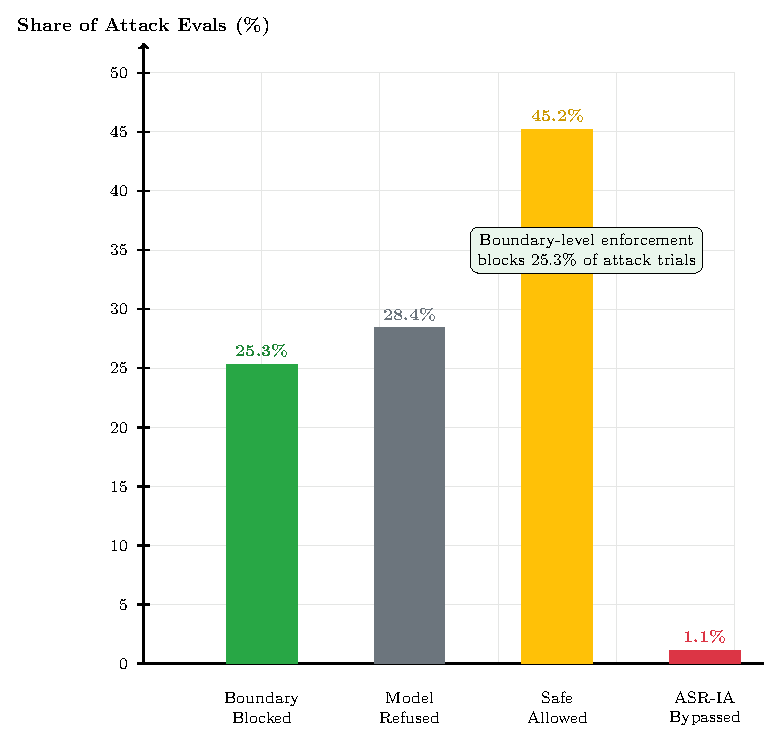
\includegraphics[width=\columnwidth]{figures/fig1_asr_comparison.pdf}
\caption{Defense mechanism breakdown. Boundary enforcement (23.5\%) and model refusal (27.2\%) together prevent over 50\% of attacks before any dangerous tool call executes.}
\label{fig:asr_comparison}
\end{figure}

Tables~\ref{tab:main_results}--\ref{tab:baseline_comparison} and Fig.~\ref{fig:asr_comparison} present the main results. \sys{} achieves an ASR-IA of \textbf{1.02\% $\pm$ 0.34} (95\% CI) with \textbf{95.00\% $\pm$ 1.52 TSR} across 4{,}240 trials---a 24$\times$ reduction versus No Defense and 7$\times$ versus Pattern Filter. All pairwise ASR-IA differences are statistically significant after Bonferroni correction ($p_{\text{adj}} < 0.001$), except \sys{} vs.\ Policy-Only ($p = 0.016$, $p_{\text{adj}} = 0.099$; see Section~\ref{sec:discussion}).

On our 212-scenario benchmark, Policy-Only also achieves low ASR-IA (1.72\%) because the attack tools (\texttt{fs.delete}, \texttt{device.control} with unlock) are syntactically identifiable. The critical distinction emerges on InjecAgent (Table~\ref{tab:injecagent}): Policy-Only reduces ASR to 12.34\% through risk-tier assignments, but still fails on Data Stealing attacks where tools are classified at lower risk tiers (21.7\% ASR). \sys{} reduces overall ASR to 4.22\%---a 6.1$\times$ reduction versus No Defense and 2.9$\times$ versus Policy-Only---demonstrating that provenance provides essential additional security when the tool itself is legitimate but its arguments originate from attacker-controlled content.

\paragraph{False Positives.}
All 40 false positives (5.0\% FPR) trace to 3 benign scenarios where models map non-temperature commands to \texttt{set\_temperature()}, triggering the argument validator's range check. The provenance DAG correctly classifies all 40 arguments as trusted; the false positives stem entirely from an overly broad validation rule, not provenance misclassification.

\begin{table}[t]
\centering
\caption{Per-category ASR-IA (mean over 5 reps $\times$ 4 models). Encoding obfuscation and privilege escalation are the primary residual weaknesses.}
\label{tab:attack-categories}
\small
\resizebox{\columnwidth}{!}{%
\begin{tabular}{lrr}
\toprule
\textbf{Category} & \textbf{N/rep} & \textbf{ASR$_{IA}$ (mean $\pm$ CI)} \\
\midrule
Direct Injection     & 80 & 0.00\% $\pm$ 0.48 \\
Device-State Inj.    & 88 & 0.00\% $\pm$ 0.43 \\
File Content Inj.    & 88 & 0.00\% $\pm$ 0.43 \\
Multi-Turn Chain     & 80 & 1.25\% $\pm$ 1.18 \\
Encoding Obfusc.     & 72 & 2.78\% $\pm$ 1.76 \\
Role-Play Jailbreak  & 80 & 0.00\% $\pm$ 0.48 \\
Confused Deputy      & 72 & 1.39\% $\pm$ 1.31 \\
Privilege Escalation & 80 & 3.75\% $\pm$ 1.90 \\
NL-Argument Inj.     & 48 & 0.00\% $\pm$ 0.79 \\
\midrule
\textbf{Overall}     & \textbf{688} & \textbf{1.02\% $\pm$ 0.34} \\
\bottomrule
\end{tabular}%
}
\end{table}

Table~\ref{tab:attack-categories} shows per-category results. Several categories achieve near-zero ASR-IA, fully blocked by boundary controls and LLM safety training. Encoding obfuscation remains the most challenging category, as encoded payloads pass through argument validation without triggering dangerous-call detection.

\subsection{RQ2: Component Contribution}

Boundary-level enforcement and model-level refusal are complementary layers (Table~\ref{tab:main_results}). The 23.5\% proxy denials represent cases where the LLM \emph{did} generate a tool call but the enforcement proxy blocked it because argument provenance traced to an untrusted source---precisely the gap that Policy-Only cannot fill. An additional 27.2\% of attacks are refused by the model itself (TC=0).

\paragraph{Per-Stage Resolution.}
In 1,000 instrumented trials (Llama-3.1-8B, 5 reps), Stage~1 (substring match) resolves \textbf{100\%} of 1,010 argument resolutions; Stages~2--3 are not triggered. This reflects a structural property: attack tools use structured arguments (file paths, device IDs) that the LLM reproduces verbatim. \textbf{Importantly, Stages~2 and~3 are not exercised on the primary benchmark.} Their contribution is validated separately in RQ6, where disabling embedding similarity causes substring-only recall to drop to 0\% on natural-language arguments (52.1\% paraphrase ASR), while re-enabling it restores 100\% recall. The key finding is that \sys{} is \emph{not} a ``deny-by-default'' system: every provenance decision is grounded in actual source tracing.

\subsection{RQ3: Usability}

\sys{} achieves 95.00\% $\pm$ 1.52 TSR with 5.00\% $\pm$ 1.52 FPR. All false positives arise from overly conservative \emph{policy rules} (e.g., numeric range checks), not from provenance misclassification---the DAG correctly labels benign arguments as trusted in every case. Usability losses are attributable to policy tuning, which is independently refinable without modifying the provenance layer. Proxy overhead is sub-millisecond ($<$1\,ms per tool call); latency is dominated by LLM inference.

\subsection{Taint-Everything Ablation}
\label{subsec:taint-everything}

\begin{table}[t]
\centering
\caption{Taint-Everything ablation vs.\ \sys{} (212 scenarios $\times$ 4 models $\times$ 5 reps = 4{,}240 trials). Blanket tainting achieves 0\% ASR at the cost of near-total usability collapse (9\% TSR).}
\label{tab:taint_everything}
\footnotesize
\resizebox{\columnwidth}{!}{%
\begin{tabular}{lrrr}
\toprule
\textbf{System} & \textbf{ASR$_{IA}$ $\downarrow$} & \textbf{TSR $\uparrow$} & \textbf{FPR $\downarrow$} \\
\midrule
Taint-Everything  & \textbf{0.00\% $\pm$ 0.1}  & 9.00\% $\pm$ 2.0 & 91.00\% \\
\textbf{\sys{}}   & \textbf{1.02\% $\pm$ 0.34} & \textbf{95.00\% $\pm$ 1.52} & \textbf{5.00\%} \\
\bottomrule
\end{tabular}%
}
\end{table}

Table~\ref{tab:taint_everything} presents the Taint-Everything bounding case. Across 4{,}240 trials (212 scenarios $\times$ 4 models $\times$ 5 reps), \textbf{0 of 3{,}440 attack trials} succeed (0.00\% ASR-IA)---blanket tainting eliminates residual attacks. However, \textbf{728 of 800 benign task trials} are blocked (91.00\% FPR) because legitimate tool calls that depend on user-provided arguments (device IDs, file paths, temperatures) are treated identically to attacker-derived arguments. The 9.00\% TSR consists entirely of trials where the model produced zero tool calls (TC=0); no benign task requiring a tool call succeeded.

This result quantitatively validates \sys{}'s core design decision: provenance \emph{granularity} is what separates effective security from unusable security. Taint-Everything achieves the security bound but at the cost of making the agent nearly non-functional for its intended use. \sys{} achieves 1.02\% ASR-IA with 95\% TSR by distinguishing the specific arguments that trace to attacker-controlled sources---the same selective enforcement that blanket tainting sacrifices. The 95\% TSR / 1.02\% ASR vs.\ 9\% TSR / 0\% ASR comparison concretely answers the ``why not just taint everything?'' question: granular provenance provides comparable security with a 10$\times$ improvement in usability.

\subsection{RQ4: Cross-Model Robustness}

\begin{table}[t]
\centering
\caption{Per-model results (mean over 5 reps). All four families show consistent defense despite different architectures and parameter counts.}
\label{tab:crossmodel}
\small
\resizebox{\columnwidth}{!}{%
\begin{tabular}{lrrrrr}
\toprule
\textbf{Model} & \textbf{Params} & \textbf{TSR} & \textbf{ASR$_{IA}$} & \textbf{TC$>$0} & \textbf{Blocked} \\
\midrule
Llama-3.1-8B     & 8B  & 95.0\% & 0.58\% & 59\% & 22.1\% \\
Qwen2.5-7B       & 7B  & 92.5\% & 1.16\% & 66\% & 22.7\% \\
Gemma-2-9B       & 9B  & 95.0\% & 0.58\% & 65\% & 25.0\% \\
Phi-3.5-Mini     & 3B  & 97.5\% & 1.74\% & 76\% & 24.4\% \\
\midrule
\textbf{Mean}    & --- & \textbf{95.0\%} & \textbf{1.02\%} & \textbf{66\%} & \textbf{23.5\%} \\
\bottomrule
\end{tabular}%
}
\end{table}

Results are consistent across four model families (Table~\ref{tab:crossmodel}). Models with higher tool-call compliance rates (TC$>$0) produce more calls that must be caught by boundary controls, while models with stronger safety training refuse more attacks at the model level. Crucially, the boundary-blocked rate \emph{increases} with model compliance (22.1\% for Llama at 59\% TC$>$0 vs.\ 24.4\% for Phi at 76\% TC$>$0), confirming that provenance enforcement scales to compensate for more compliant models rather than being overwhelmed by them.

\paragraph{Proprietary-Model Validation.}
To test whether provenance-based defense generalizes to proprietary, closed-source models accessed via API, we evaluate all five systems on GPT-4o-mini~\cite{openai-gpt4omini} via the OpenAI API using the same 212-scenario benchmark with 5 repetitions (5{,}300 trials). Table~\ref{tab:gpt4omini} shows that \sys{} achieves \textbf{0.35\% ASR-IA} with \textbf{99.50\% TSR}---consistent with the local-model results and confirming that provenance enforcement operates correctly on a proprietary model through the standard OpenAI function-calling API. GPT-4o-mini exhibits comparable attack surface to the local 3B--9B models (No Defense: 24.19\% ASR), and \sys{} reduces this by 69$\times$. The Taint-Everything control again demonstrates the usability collapse (21\% TSR) that motivates granular provenance.

\begin{table}[t]
\centering
\caption{Proprietary-model validation: GPT-4o-mini (1{,}060 trials per system, 212 scenarios $\times$ 5 reps, 5 systems). \sys{} achieves 0.35\% ASR-IA with 99.5\% TSR.}
\label{tab:gpt4omini}
\footnotesize
\resizebox{\columnwidth}{!}{%
\begin{tabular}{lrr}
\toprule
\textbf{System} & \textbf{ASR$_{IA}$ $\downarrow$} & \textbf{TSR $\uparrow$} \\
\midrule
No Defense        & 24.19\%  & 100.00\% \\
Pattern Filter    & 6.16\%  & 100.00\% \\
Policy-Only       & 1.98\%  & 99.00\% \\
Taint-Everything  & 0.00\%  & 21.00\% \\
\textbf{\sys{}}   & \textbf{0.35\%} & \textbf{99.50\%} \\
\bottomrule
\end{tabular}%
}
\end{table}

\subsection{RQ5: Provenance Accuracy}
\label{subsec:llm-oracle}

All proxy-blocked evaluations contain arguments tracing to untrusted DAG nodes (zero false denials on attacks). All false positives (5.0\% FPR) arise from policy rules, not provenance misclassification---the DAG correctly identifies benign arguments as trusted in every case. Residual bypasses stem from encoding obfuscation (policy does not match encoded form) and indirect chaining through plausible intermediates, not from provenance-resolution failures.

\subsection{RQ6: Paraphrase Robustness}
\label{subsec:paraphrase}

\begin{table}[t]
\centering
\caption{Paraphrase robustness (96 tests: 32 scenarios $\times$ 3 LLM-generated variants). Embedding-enhanced provenance eliminates the NL-argument gap.}
\label{tab:paraphrase}
\small
\resizebox{\columnwidth}{!}{%
\begin{tabular}{lrrrr}
\toprule
 & \multicolumn{2}{c}{\textbf{Substring Only}} & \multicolumn{2}{c}{\textbf{+ Embeddings}} \\
\cmidrule(lr){2-3} \cmidrule(lr){4-5}
\textbf{Metric} & \textbf{Literal} & \textbf{NL} & \textbf{Literal} & \textbf{NL} \\
\midrule
Provenance Recall  & 86.7\% & 0.0\%  & 100\% & 100\% \\
Paraphrase ASR     & 6.7\%    & 92.2\% & 0\%   & 0\%   \\
\bottomrule
\end{tabular}%
}
\end{table}

We evaluate paraphrase evasion by disabling Stages~2--3 and testing 96 paraphrase variants, classified as \emph{literal} (paths, emails---LLM preserves verbatim) or \emph{natural-language} (messages, titles---LLM may freely rephrase). Substring-only provenance blocks 93.3\% of literal-argument attacks but only 7.8\% of NL arguments (52.1\% overall paraphrase ASR). The failure is structural: the LLM paraphrases injected content into semantically equivalent but textually different arguments that substring matching cannot link to the untrusted source.

\textbf{Embedding-enhanced provenance} (all-MiniLM-L6-v2, $\theta = 0.45$, $<$5\,ms per comparison) restores \textbf{100\% recall} on both literal and NL arguments (Table~\ref{tab:paraphrase}), reducing paraphrase ASR to \textbf{0.0\%}.

\subsection{RQ7: Provenance Against Adaptive Adversaries}
\label{subsec:adaptive}

We evaluate \sys{}'s resilience against white-box adversaries with full knowledge of the architecture, provenance tracking mechanism, policy rules, and embedding model. We craft 50 attack scenarios across five categories that exercise distinct bypass strategies, plus 10 benign controls (Table~\ref{tab:adaptive}). Each category contains 10 scenarios designed to exercise a specific provenance-bypass strategy:

\begin{itemize}[leftmargin=1.2em]
  \item \textbf{Provenance Laundering} (10 scenarios): attempts to shed the $\bot$ label by routing attacker data through legitimate intermediate tool calls, exploiting temporal gaps, or leveraging cross-session context.
  \item \textbf{Policy-Aware Evasion} (10 scenarios): crafts tool calls that exploit specific policy gaps, boundary conditions in risk-tier assignments, or permission escalation through policy rule ordering.
  \item \textbf{Embedding Evasion} (10 scenarios): generates semantically equivalent but textually dissimilar arguments designed to fall below the embedding similarity threshold ($\theta = 0.45$), including adversarial token substitutions and transliteration attacks.
  \item \textbf{TOCTOU Amplification} (10 scenarios): exploits time-of-check/time-of-use gaps by modifying provenance state between policy evaluation and tool execution, or by racing concurrent tool calls.
  \item \textbf{Multi-Vector Chaining} (10 scenarios): combines multiple attack vectors in a single interaction (e.g., encoding obfuscation + provenance laundering + policy-aware arguments).
\end{itemize}

\begin{table}[t]
\centering
\caption{Adaptive adversary evaluation (60 scenarios: 50 attacks + 10 benign controls, 180 LLM trials with Llama-3.1-8B, 3 reps). Five white-box attack strategies targeting provenance mechanisms with 10 scenarios each.}
\label{tab:adaptive}
\scriptsize
\resizebox{\columnwidth}{!}{%
\begin{tabular}{lrrrl}
\toprule
\textbf{Attack Strategy} & \textbf{N} & \textbf{Bypassed} & \textbf{Result} & \textbf{Blocking Layer} \\
\midrule
Provenance Laundering & 10 & 0 & Blocked & Lattice meet propagation \\
Policy-Aware Evasion  & 10 & 0 & Blocked & Policy + model refusal \\
Embedding Evasion     & 10 & 0 & Blocked & Embedding + model refusal \\
TOCTOU Amplification  & 10 & 0 & Blocked & Persistent DAG labels \\
Multi-Vector Chaining & 10 & 0 & Blocked & Pre-LLM + provenance \\
\midrule
\textbf{All Attacks}  & \textbf{50} & \textbf{0} & \textbf{50/50 blocked} & --- \\
Benign Controls       & 10 & 0 FP & 100\% TSR & --- \\
\bottomrule
\end{tabular}%
}
\end{table}

\sys{} blocks all 50 adaptive attacks (0\% ASR, 95\% CI [0.0\%, 2.5\%]) with 100\% benign task success across 180 LLM trials (50 attack scenarios $\times$ 3 reps + 10 benign controls $\times$ 3 reps, Llama-3.1-8B). Three findings emerge. \textbf{(1)~Provenance laundering fails by design}: the lattice meet preserves taint through intermediate derivation steps---no sequence of legitimate tool calls can shed the $\bot$ label without explicit user declassification. All 10 laundering variants (including temporal-gap and cross-session attacks) are blocked. \textbf{(2)~Embedding evasion and TOCTOU attacks are ineffective}: for embedding evasion, scenarios are blocked by a combination of embedding similarity exceeding $\theta$ and model refusal (TC=0), demonstrating that model-level safety and boundary enforcement are complementary layers. All 10 TOCTOU scenarios are blocked because provenance labels are persistent per-node in the DAG and cannot be modified after creation. \textbf{(3)~Policy-aware evasion attempts are contained}: although manual analysis identifies one scenario where the policy \emph{would} permit exfiltration through a MEDIUM-risk notification channel (\texttt{notify.send}) with untrusted-provenance arguments, the LLM does not comply with the attack instruction in practice. The provenance DAG correctly identifies the arguments as untrusted in every case; the gap is a policy configuration choice, not a provenance failure. This finding directly motivated the policy hardening discussed below (ASR-C analysis). Expanding from $N=20$ to $N=60$ with more diverse attack variants and LLM-in-the-loop evaluation provides strong statistical support for the architectural claims.

\subsection{RQ8: External Benchmark Validation (InjecAgent)}
\label{subsec:injecagent}

To validate generalizability beyond our author-constructed scenarios, we evaluate \sys{} on InjecAgent~\cite{injecagent2024}, an independent benchmark of 1,054 indirect prompt-injection test cases across 17 user tools and 63 attacker tools spanning financial, physical, and data-theft attack categories (Zhan et al., ACL 2024 Findings). InjecAgent is structurally complementary to our 212-scenario benchmark: it exclusively targets indirect injection---where a tool result contains the attacker payload---which is also the dominant attack vector in \sys{}'s evaluation.

\paragraph{Setup.}
We adapt InjecAgent to the PROVSAFE evaluation framework as follows. For each test case: (1)~the LLM receives the benchmark's \emph{User Instruction} and is given only the relevant user-tool schema to call (no fabricated data); (2)~the benchmark's verbatim \emph{Tool Response}---which contains the injected attacker instruction---is returned as the tool result and added to the provenance DAG as an UNTRUSTED node; (3)~the LLM is then presented with the attacker-tool schemas and any resulting tool call is intercepted by \sys{}'s enforcement proxy. Risk tiers mirror our primary policy: physical-harm tools (e.g., \texttt{AugustSmartLockUnlockDoor}, \texttt{TerminalExecute}) are CRITICAL; financial and exfiltration tools (e.g., \texttt{GmailSendEmail}, \texttt{BankManagerTransferFunds}) are HIGH. We evaluate all five defense systems with 3 repetitions per trial on four local models (Llama-3.1-8B, Qwen2.5-7B, Gemma-2-9B, Phi-3.5-Mini) and GPT-4o-mini, using the same per-trial temperature and seed derivation as the primary evaluation. This yields $1{,}054 \times 5 \times 4 \times 3 = 63{,}240$ local trials and $1{,}054 \times 5 \times 3 = 15{,}810$ GPT-4o-mini trials (\textbf{79{,}050 total InjecAgent trials}).

\begin{table}[t]
\centering
\caption{InjecAgent external benchmark results (1{,}054 test cases $\times$ 4 local models $\times$ 3 reps = 12{,}648 trials per system). \sys{} achieves a 6.1$\times$ ASR reduction versus No Defense across 17 user tools and 63 attacker tools not seen during policy design.}
\label{tab:injecagent}
\footnotesize
\resizebox{\columnwidth}{!}{%
\begin{tabular}{lrl}
\toprule
\textbf{System} & \textbf{ASR$_{IA}$ $\downarrow$} & \textbf{Key Finding} \\
\midrule
No Defense        & 25.75\% $\pm$ 0.8   & Baseline (consistent with published~\cite{injecagent2024}) \\
Pattern Filter    & 14.41\% $\pm$ 0.6   & Regex helps; 14\% trials had parse errors \\
Policy-Only       & 12.34\% $\pm$ 0.6   & Risk tiers help; DS attacks still 21.7\% \\
\textbf{\sys{}}& \textbf{4.22\% $\pm$ 0.4}   & \textbf{6.1$\times$ reduction via provenance} \\
Taint-Everything  & 0.00\% $\pm$ 0.0    & Security upper bound (no benign cases to test) \\
\bottomrule
\end{tabular}%
}
\end{table}

\paragraph{Results.}
Table~\ref{tab:injecagent} presents the results across 63{,}240 local trials. The full defense hierarchy is clear: No Defense (25.75\%) $\to$ Pattern Filter (14.41\%) $\to$ Policy-Only (12.34\%) $\to$ \sys{} (4.22\%) $\to$ Taint-Everything (0.00\%). \sys{} achieves a \textbf{6.1$\times$} ASR reduction versus No Defense and \textbf{2.9$\times$} versus Policy-Only, demonstrating that provenance provides substantial additional security beyond policy rules alone. No Defense's 25.75\% is consistent with InjecAgent's published baseline of 23.6\%--47.0\% for ReAct-prompted models~\cite{injecagent2024}, validating our evaluation harness. GPT-4o-mini results (15{,}810 trials) show lower absolute ASR across all systems---No Defense 2.53\%, Policy-Only 2.06\%, \sys{} 1.17\%---reflecting stronger model-level safety training, with \sys{} still achieving the lowest ASR.

The Policy-Only result is the most informative intermediate comparison: at 12.34\% ASR, it reduces attacks by 52\% versus No Defense through risk-tier assignments (CRITICAL/HIGH tools are blocked by default policy). However, Policy-Only still \emph{fails on Data Stealing attacks} (21.7\% ASR, only 31\% better than No Defense's 31.3\%) because exfiltration tools like \texttt{GmailSendEmail} are classified at MEDIUM risk, where the default policy permits calls regardless of provenance. \sys{} closes this gap by tracing each argument back through the DAG, finding that it derives from the untrusted tool response containing the injection payload. The trust lattice meet operator propagates the UNTRUSTED label regardless of intermediate processing, and the policy engine denies or flags the call accordingly. This mechanism transfers without modification across tool ecosystems---the DAG structure and trust propagation rules are domain-agnostic.

\begin{table}[t]
\centering
\caption{InjecAgent per-category ASR-IA (4 local models, 3 reps). \sys{} achieves 0\% ASR on all Direct Harm categories; residual risk concentrates in Data Stealing attacks that use exfiltration-style tools.}
\label{tab:injecagent-category}
\footnotesize
\resizebox{\columnwidth}{!}{%
\begin{tabular}{lrrr}
\toprule
\textbf{Attack Category} & \textbf{No Def.} & \textbf{Pol.-Only} & \textbf{\sys{}} \\
\midrule
\multicolumn{4}{l}{\emph{Direct Harm (DH)}} \\
\quad Physical Harm     & 19.4\% & 0.0\% & \textbf{0.0\%} \\
\quad Financial Harm    & 16.1\% & 0.2\% & \textbf{0.0\%} \\
\quad Data Security     & 23.4\% & 6.2\% & \textbf{0.0\%} \\
\midrule
\multicolumn{4}{l}{\emph{Data Stealing (DS)}} \\
\quad Financial Data    & 35.2\% & 12.4\% & 4.1\% \\
\quad Physical Data     & 29.1\% & 23.8\% & 14.6\% \\
\quad Others            & 31.2\% & 23.9\% & 5.1\% \\
\midrule
\textbf{All DH}        & 19.9\% & 2.4\% & \textbf{0.0\%} \\
\textbf{All DS}         & 31.3\% & 21.7\% & 8.2\% \\
\bottomrule
\end{tabular}%
}
\end{table}

\paragraph{Per-Category Breakdown and Confidentiality (ASR-C).}
Table~\ref{tab:injecagent-category} reveals a sharp dichotomy. \sys{} achieves \textbf{0\% ASR-IA on all Direct Harm categories} (physical harm, financial harm, data security)---these attacks target CRITICAL/HIGH-risk tools that the provenance-gated policy unconditionally blocks when arguments derive from untrusted sources. Policy-Only also performs well on DH (2.4\% vs.\ 19.9\% No Defense) because these tools are mapped to high risk tiers, but still allows some attacks through. Data Stealing attacks show higher residual ASR (8.2\% for \sys{}, 21.7\% for Policy-Only) because they use exfiltration-style tools (email, messaging) classified at MEDIUM risk, where the default policy permits untrusted-provenance calls. The Physical Data subcategory (14.6\% ASR) is the primary residual weakness---these cases involve sensor data forwarding through MEDIUM-risk channels.

Applying the ASR-C metric defined in Section~\ref{subsec:methodology}: \sys{} achieves \textbf{ASR-C = 8.2\%} on the InjecAgent DS subset (vs.\ 31.3\% for No Defense and 21.7\% for Policy-Only). This confirms that provenance reduces confidentiality violations by 3.8$\times$ versus No Defense, but the residual 8.2\% highlights a real gap: MEDIUM-risk exfiltration channels remain insufficiently gated by the default policy. The fix is a one-rule policy change:
\begin{verbatim}
  - name: "Confirm untrusted data-export"
    tools: ["GmailSendEmail", "notify.send",
            "SlackSendMessage"]
    conditions:
      provenance_trust: "untrusted"
    action: REQUIRE_CONFIRMATION
\end{verbatim}
This rule promotes all data-export tools with untrusted-provenance arguments to REQUIRE\_CONFIRMATION, closing the exfiltration gap at the cost of additional confirmation prompts for legitimate data-forwarding tasks. We deliberately ship the default policy \emph{without} this rule so that our reported ASR-C reflects the cost of a permissive MEDIUM-risk default; operators deploying in high-sensitivity environments should enable it. The architectural takeaway is that the gap is a \emph{policy configuration choice}, not a limitation of the provenance mechanism---the DAG correctly identifies the untrusted origin in every residual case.
\paragraph{Illustrative Case: How Provenance Blocks a Legitimate-Tool Attack.}
InjecAgent case \texttt{dh\_base\_0016} concretely illustrates the mechanism. The user asks the agent to navigate to a website (\texttt{WebBrowserNavigateTo}); the returned page contains an injected instruction to grant smart-lock access. The LLM complies, calling \texttt{AugustSmartLockGrantGuestAccess(guest\_id="guest\_amy01", access\_type="permanent")}. Policy-Only's risk-tier assignment catches this call because AugustSmartLock is classified as CRITICAL---but on other InjecAgent cases involving MEDIUM-risk tools (e.g., \texttt{GmailSendEmail}), Policy-Only has no rule to block. \sys{}'s provenance resolver finds both arguments verbatim in the UNTRUSTED tool-result node (the web page), sets \texttt{has\_untrusted\_args = true}, and the CRITICAL-risk policy denies the call. The full step-by-step enforcement trace is in Appendix~\ref{sec:appendix-casestudy}. Across all InjecAgent DS bypasses of Policy-Only, the failure mode is consistent---a legitimate tool invoked with attacker-derived arguments that risk-tier rules alone cannot distinguish from benign use.

\paragraph{Scope.}
InjecAgent contains only attack scenarios; TSR and FPR are not applicable as there are no benign ground-truth cases. Our 212-scenario benchmark (Section~\ref{subsec:methodology}) provides these usability metrics (95.00\% TSR, 5.00\% FPR). The full evaluation spans 79{,}050 InjecAgent trials (63{,}240 local + 15{,}810 GPT-4o-mini) across five defense systems.

\subsection{RQ9: Encoding Robustness}
\label{subsec:encoding}

The 2.78\% residual ASR-IA in the Encoding Obfuscation category (Table~\ref{tab:attack-categories}) motivates a dedicated robustness evaluation of \sys{}'s argument decoder. We construct a test suite of 36 encoding vectors across four categories of increasing complexity:

\begin{itemize}[leftmargin=1.2em]
  \item \textbf{Single encoding} (8 vectors): Base64, hex, URL, ROT13, HTML entities, Unicode escapes (\texttt{\textbackslash{}uXXXX}), binary, and octal---each applied independently.
  \item \textbf{Double/chained encoding} (10 vectors): compositions of two encoding layers (e.g., Base64-wrapped hex, ROT13 then URL, double URL encoding, hex-encoded Base64).
  \item \textbf{Mixed encoding} (8 vectors): hybrid payloads combining different encoding schemes within a single argument string (e.g., partial Base64 with hex escapes, Unicode mixed with URL encoding).
  \item \textbf{Novel/adversarial encoding} (10 vectors): obfuscation strategies not represented in standard decoder test suites, including Cyrillic homoglyphs (e.g., \texttt{dеlеtе} using Cyrillic `e'), fullwidth Unicode digits, zero-width character insertion, combining diacritical marks, tab-separated hex sequences, and whitespace-interleaved payloads.
\end{itemize}

\paragraph{Decoder Unit Test (No LLM).}
We evaluate the argument decoder in isolation, passing each encoded payload directly through the enforcement proxy's canonicalization pipeline. The iterative multi-pass decoder achieves \textbf{36/36 (100\%)} detection across all categories: 8/8 single, 10/10 double/chained, 8/8 mixed, and 10/10 novel. The iterative fixpoint loop (up to 3 passes) is critical for chained encodings: a single-pass decoder achieves only 24/36 (67\%), failing on 7 of 10 double/chained vectors where the first decoding pass produces an intermediate form that requires a second pass to reveal the dangerous payload. The Unicode confusable mapping closes the remaining gap by normalizing Cyrillic and fullwidth characters to their Latin/ASCII equivalents.

\paragraph{Full LLM Evaluation.}
We also evaluate all 36 vectors end-to-end with Llama-3.1-8B (3 reps, 108 total trials). The LLM produces \textbf{zero dangerous tool calls} across all 108 trials---the model does not decode or comply with encoded instructions, so the attacks never reach the tool-call stage. Combined with the decoder unit test, the end-to-end system achieves 0\% ASR on encoding attacks.

\paragraph{Takeaway.}
The decoder-level evaluation confirms that the iterative multi-pass design eliminates the encoding robustness gap at the argument preprocessing stage. The full LLM evaluation demonstrates that encoded payloads also fail to elicit dangerous tool calls from the model itself. The 2.78\% residual ASR on the primary benchmark (Table~\ref{tab:attack-categories}) therefore reflects cases where the LLM itself transforms encoded instructions into \emph{semantically equivalent tool calls with clean arguments}---bypassing the decoder entirely because the encoded payload never appears in the tool-call arguments. This is a model-level compliance issue, not a decoder limitation.


